\section{格林Green公式}

本节讨论格林Green公式。
Green公式是二维平面的二重积分和边界积分的关系,是后续两个公式的“预热”。

本节要点:
\begin{itemize}
    \item 掌握Green公式的概念。
\end{itemize}

%============================================================
\subsection{格林Green公式的概念}

\begin{definition}[Green公式]
假设二维平面中有单连通区域$D$,其正向边界$L$分段光滑,$\boldsymbol{f}\left( \boldsymbol{p} \right) =\left( P\,\,Q \right) ^T$是定义在二维平面上的向量值函数,且$P,Q$在$D$上有一阶连续偏导数,则有:
\[
\oint\limits_L{\boldsymbol{f}^T\boldsymbol{dl}}=\oint\limits_L{Pdx+Qdy}=\iint\limits_D{\left( \frac{\partial Q}{\partial x}-\frac{\partial P}{\partial y} \right) dxdy}
\]
上述公式称为{\bf Green公式}。
若假设$D$为复连通区域,其正向外边界为$L_1$,正向内边界为$L_2$,则有:
\[
\oint\limits_{L_1}{\boldsymbol{f}^T\boldsymbol{dl}}+\oint\limits_{L_2}{\boldsymbol{f}^T\boldsymbol{dl}}=\iint\limits_D{\left( \frac{\partial Q}{\partial x}-\frac{\partial P}{\partial y} \right) dxdy}
\]
\end{definition}

\begin{figure}[h]
\centering
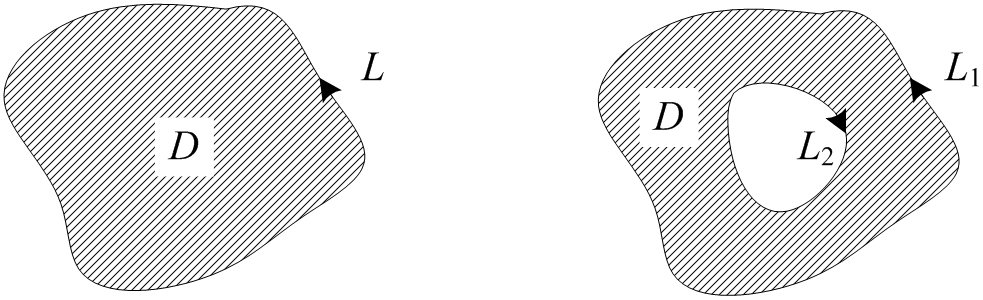
\includegraphics[height=2.5cm]{11.1.png}
\end{figure}




